\documentclass[10pt,a4paper]{article}
\usepackage[T1]{fontenc}\usepackage{lmodern,amsmath,tikz,xurl}
\usepackage[margin=22mm]{geometry}\usetikzlibrary{arrows.meta,positioning}
\title{Reusable GMRES workspace}\date{Created-at: 2026-10-25 15:12 CET}
\begin{document}\maketitle
\textbf{Authorization and owner.} The user requests a mathematical summary first,
then the proposed allocation/copy fixes. Tensor's existing hymeko\_numerics owns
the one GMRES engine; Core retains IR ownership and Graph retains PageRank
normalization and its independent L1 certificate. No numerical dependencies are added.
Existing unrelated tensor/linalg work is preserved.

\textbf{Design.} Keep gmres as the existing allocating facade, delegating to a
caller-owned GmresWorkspace. Store basis vectors contiguously, reuse the small
Hessenberg/rotation/back-substitution buffers, construct Arnoldi work in place,
and avoid constructing an unused next basis vector at cycle/budget termination.
Expose typed relative/absolute tolerance through a configuration value; report
the actual relative residual. Preserve scalar arithmetic order and restart semantics.
Do not change preconditioning, orthogonalization strategy, parallelism or defaults.

\textbf{Acceptance.} Focused existing solver, diffusion and port-Hamiltonian
correctness checks, independent dense-oracle checks, frozen pre-change arithmetic
comparison, boundary/reuse tests, and deterministic allocation-count assertions.
Graph integration uses the same owner; its pinned dependency must remain portable.
A temporary command-line provider override may verify local integration but is
not a published dependency. No commit/push is authorized in this request.

\textbf{Scope and risks.} New workspace API and its tests, existing gmres facade,
targeted client integration and documentation. Floating-point reduction ordering,
stale buffers, incomplete restarts and falsely reported convergence are the main
risks. Capacity reuse preserves memory across calls; it does not remove O(nm)
basis storage. No new benchmark or profiler is run. ETA: 45--75 minutes for the
PDF, implementation and correctness checks, depending on integration constraints.

\textbf{Checkout.} Tensor feat/virtual-operators at 9317ecf and Graph
feat/newest-core at 57e111c match their freshly fetched upstreams. Tensor main has
one additional merge commit with an identical tree. Reuse both existing dirty
checkouts; preserve unrelated changes. A rollback consists only of this task's
named paths/hunks, not a reset or stash.

\begin{center}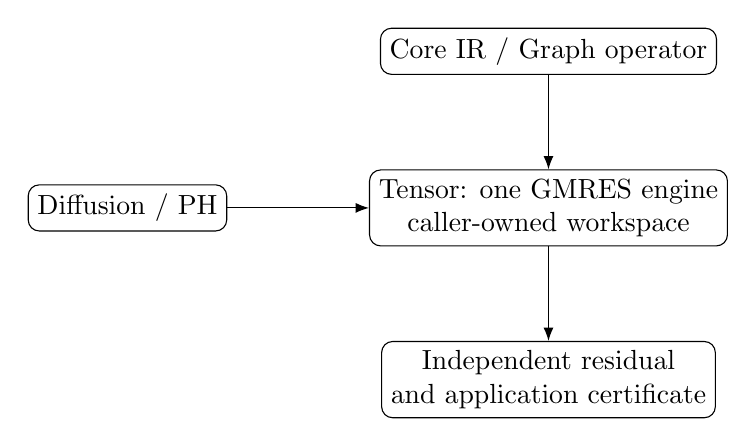
\begin{tikzpicture}[node distance=12mm,box/.style={draw,rounded corners,align=center}]
\node[box] (graph) {Core IR / Graph operator};
\node[box,below=of graph] (solver) {Tensor: one GMRES engine\\caller-owned workspace};
\node[box,left=18mm of solver] (physics) {Diffusion / PH};
\node[box,below=of solver] (check) {Independent residual\\and application certificate};
\draw[-{Latex}] (graph)--(solver);\draw[-{Latex}] (physics)--(solver);\draw[-{Latex}] (solver)--(check);
\end{tikzpicture}\end{center}

\textbf{Outcome, 25 October 2026.} The four-page mathematical summary was built
before production changes. All 61 focused correctness tests pass, including
144 frozen bitwise cases and eight full-size Graph inputs. Warm workspace and
PageRank calls allocate nothing in the deterministic checks. Tensor duplication
fell from 155/2436 to 153/2416; Graph remains 554/9201. The temporary Graph
provider override is checkout-local, excluded from Git and documented in README;
versioned provider publication and lockfile finalization remain pending. No
commit, push or new latency measurement was performed. Detailed receipts and
the one-page implementation PDF are in
\path{reports/2026-10-25-gmres-workspace/}.
\textbf{Publication, 25 October 2026, 17:47 CET.} The user now authorizes commit
and upload. Publish the named numerics files and mathematics note to Tensor's
existing origin feature branch, then pin that exact revision in Graph and remove
the checkout-local override. Verify the staged source exports and versioned
dependency, preserving the unrelated dense-linear-algebra edits. Do not merge
main or change GitHub visibility. Generated evidence remains in the Samba archive.
\end{document}
